%%% diambil dari Form A
\newpage
\begin{center}
{\normalfont\Large\bfseries\expandafter{SYARAT YANG HARUS DIPENUHI OLEH MAHASISWA SESUDAH DINYATAKAN LULUS TESIS}}
\par\nobreak
\end{center}

\vspace{1cm}
\begin{center}
{\normalfont\large\bfseries\expandafter{LIST PERSYARATAN PROGRAM STUDI S2 ILMU KOMPUER}}
\par\nobreak
\end{center}

\vspace{.5cm}
\begin{bfseries}
\begin{tabbing}
NAMA 	\= : \@fullname \\ [0.2cm]
NIM 	\> : \@idnum \\ [0.2cm]
PRODI 	\> : \@program
\end{tabbing}
\end{bfseries}

\renewcommand{\arraystretch}{1.5}
\begin{center}
\begin{tabular}{|c|m{1cm}|m{13cm}|}
\hline
1 & 
\vspace{0.2cm} 

\begin{tikzpicture} 
\draw (0,0) rectangle (1,1); 
\end{tikzpicture} 
& Hard copy Tesis, Publikasi dan Summary \\ \hline
2 & 
\vspace{0.2cm} 

\begin{tikzpicture} 
\draw (0,0) rectangle (1,1); 
\end{tikzpicture} 
& Form S2-14 dan S2-15 yang sudah di tandatangani masing-masing 2 lembar \\ \hline
3 & 
\vspace{0.2cm} 

\begin{tikzpicture} 
\draw (0,0) rectangle (1,1); 
\end{tikzpicture} 
& Biodata Mahasiswa ditempel 2 buah foto warna 3$\times$4 dan 4$\times$6, dengan format terlampir \\ \hline
4 & 
\vspace{0.2cm} 

\begin{tikzpicture} 
\draw (0,0) rectangle (1,1); 
\end{tikzpicture} 
& Foto copy Bukti Penyerahan CD Tesis dan Surat Keterangan Bebas Pinjam Pustaka (yang Asli untuk syarat Yudisium) dari: \vfill
\hspace{.3cm} 1. Perpustakaan Pusat \vfill
\hspace{.3cm} 2. Perpustakaan Fakultas \\ \hline
5 & 
\vspace{0.2cm} 

\begin{tikzpicture} 
\draw (0,0) rectangle (1,1); 
\end{tikzpicture} 
& CD Tesis Lengkap = 2 buah yang berisi : Tesis beserta Software program, Naskah Publikasi, Abstract dan Intisari Lepas, Pas Foto Warna dan Summary Indonesia dan English dengan Format \textbf{DOC} dan \textbf{PDF} \\ \hline
6 & 
\vspace{0.2cm} 
\begin{tikzpicture} 
\draw (0,0) rectangle (1,1); 
\draw (0,0) -- (1,1) -- (0,1) -- (1,0);
\end{tikzpicture} 
& Melunasi pembayaran Acara Pelepasan Wisuda Pascasarjana FMIPA sebesar \vfill \textbf{Rp. 200.000,-} (\textit{Dua ratus ribu rupiah}) melalui Program Studi. \\ \hline
7 & 
\vspace{0.2cm} 

\begin{tikzpicture} 
\draw (0,0) rectangle (1,1); 
\end{tikzpicture} 
& Abstract dan Intisari lepas masing-masing 1 lembar \\ \hline
8 & 
\vspace{0.2cm} 

\begin{tikzpicture} 
\draw (0,0) rectangle (1,1); 
\end{tikzpicture} 
& Halaman Pengesahan Tesis Asli 1 lembar\\ \hline
9 & 
\vspace{0.2cm} 

\begin{tikzpicture} 
\draw (0,0) rectangle (1,1); 
\end{tikzpicture} 
& Mengirimkan scan Halaman Pengesahan Tesis ke email \textit{mkom@ugm.ac.id} \\ \hline
\end{tabular}
\end{center}


% diambil dari Form A
\newpage
\begin{center}
{\normalfont\large\bfseries\expandafter{LIST PERSYARATAN YUDISIUM JENJANG S2 FMIPA UGM}}
\par\nobreak
\end{center}

\vspace{.1cm}
\begin{bfseries}
\begin{tabbing}
NAMA 	\= : \@fullname \\ [0.2cm]
NIM 	\> : \@idnum \\ [0.2cm]
PRODI 	\> : \@program
\end{tabbing}
\end{bfseries}

\begin{center}
\begin{tabular}{|c|m{1cm}|m{13cm}|}
\hline
1 & 
\vspace{0.2cm} 

\begin{tikzpicture} 
\draw (0,0) rectangle (1,1); 
\end{tikzpicture} 
& Surat Permohonan Yudisium (Form permohonan bisa didapatkan di Prodi). \\ \hline
2 & 
\vspace{0.2cm} 

\begin{tikzpicture} 
\draw (0,0) rectangle (1,1); 
\end{tikzpicture} 
& Transkrip mata kuliah (dari Palawa) yang sudah ditandatangani pejabat program studi. \\ \hline
3 & 
\vspace{0.4cm} 

\begin{tikzpicture} 
\draw (0,0) rectangle (1,1); 
\end{tikzpicture} 
& Fotokopi Surat Keterangan Lulus AcEPT/TOEFL dan PAPs/TPA dari lembaga yang diakui oleh UGM masing-masing 1 lembar. \\ \hline
4 & 
\vspace{0.2cm} 

\begin{tikzpicture} 
\draw (0,0) rectangle (1,1); 
\end{tikzpicture} 
& Bukti penyerahan tesis melalui Unggah Mandiri (upload) di alamat \vfill \textit{https://unggah.etd.ugm.ac.id} (dengan menngunakan akun email UGM). \vfill
\vspace{0.2cm}
Untuk keterangan lebih lanjut mengenai persyaratan point ini dapat dilihat pada \vfill "Pengumumnan Wisuda Program S2/Spesialis/S3" di \textit{http://akademik.ugm.ac.id} \\ \hline
5 & 
\vspace{0.2cm} 

\begin{tikzpicture} 
\draw (0,0) rectangle (1,1); 
\end{tikzpicture} & 
Surat Pernyataan (bermeterai Rp 6.000,-) tidak memiliki tanggungan pinjaman buku di Perpustakaan di seluruh UGM dan alat-alat di laboratorium di lingkungan UGM dengan dilampiri: \vfill
-- Surat keterangan bebas pinjam buku Perpustakaan Pusat UGM \vfill
-- Surat keterangan bebas pinjam buku Perpustakaan Fakultas/Program Studi. \vfill
-- Surat keterangan bebas pinjam alat laboratorium (LPPT dan Program Studi). \\ \hline
6 & 
\vspace{0.2cm} 
\begin{tikzpicture} 
\draw (0,0) rectangle (1,1);
\end{tikzpicture} 
& Formulir S2-14, S2-15, Berita Acara Ujian Tesis (dari Prodi) masing-masing 1 lembar. \\ \hline
7 & 
\vspace{0.2cm} 

\begin{tikzpicture} 
\draw (0,0) rectangle (1,1); 
\end{tikzpicture} 
& CD yang berisi: \vfill
-- Scan Halaman Pengesahan Tesis format \textbf{PDF}. \vfill
-- Naskah Publikasi lengkap masing-masing dalam 1 file dengan format \textbf{DOC} dan \textbf{PDF (bukan latex)} \vfill
Disimpan dalam 1 CD dan dalam file yang terpisah. \vfill

\begin{bfseries}
\vspace{0.2cm}
Tambahan: \vfill
Bagi mahasiswa yang akan submit ke Berkala MIPA dapat menggunakan \vfill alamat: \textit{https://journal.ugm.ac.id/bimipa} dan mohon untuk dapat melampirkan bukti sudah submit (di-scan dan disimpan dalam file terpisah di CD di atas). \end{bfseries} \\ \hline
\end{tabular}
\end{center}

\vspace{0.5cm}

\begin{bfseries}
\noindent
Catatan: \linebreak
Mohon persyaratan di atas dikumpulkan di Program Studi dengan terlebih dahulu di-urutkan sesuai urutan di atas dan tidak perlu distaples (cukup dijepit paper clip).
\end{bfseries}


% diambil dari Form A
\newpage
\begin{center}
{\normalfont\large\bfseries\expandafter{LIST PERSYARATAN WISUDA JENJANG S2 FMIPA UGM}}
\par\nobreak
\end{center}

\vspace{.1cm}
\begin{bfseries}
\begin{tabbing}
NAMA 	\= : \@fullname \\ [0.2cm]
NIM 	\> : \@idnum \\ [0.2cm]
PRODI 	\> : \@program
\end{tabbing}
\end{bfseries}

\begin{center}
\begin{tabular}{|c|m{1cm}|m{13cm}|}
\hline
1 & 
\vspace{0.2cm} 

\begin{tikzpicture} 
\draw (0,0) rectangle (1,1); 
\end{tikzpicture} 
& Pas foto 3$\times$4 hitam putih terbaru = 2 lembar lepas, \textbf{dimasukkan ke dalam plastik berklip.} \vfill
-- Foto berwarna dasar gelap, \textbf{kertas foto dof} (agar stempel cap dinas Fakultas bisa melekat); \vfill
-- Posisi badan tegap menghadap ke depan, posisi badan tidak boleh miring; \vfill
-- Khusus laki-laki diwajibkan memakai pakaian sipil lengkap (jas berdasi), \vfill \hspace{.17cm} perempuan menyesuaikan; \vfill
-- Kedua daun telinga harus kelihatan bagi yang tidak berjilbab dan tidak \vfill \hspace{.17cm} memakai kaca mata hitam. \\ \hline
2 & 
\vspace{0.2cm} 

\begin{tikzpicture} 
\draw (0,0) rectangle (1,1); 
\end{tikzpicture} 
& Kartu mahasiswa \textbf{\underline{ASLI}} (yang masih berlaku) atau Kartu Mahasiswa (KTM) yang sudah ditutup (dilubangi) oleh BNI, \textbf{dimasukkan ke dalam plastik berklip.} \\ \hline
3 & \vspace{0.2cm} 
\begin{tikzpicture} \draw (0,0) rectangle (1,1); \end{tikzpicture} & Legalisir Surat Keterangan Lulus AcEPT/TOEFL dan PAPs/TPA dari lembaga yang diakui oleh UGM masing-masing 1 lembar \\ \hline
4 & 
\vspace{0.2cm} 

\begin{tikzpicture} 
\draw (0,0) rectangle (1,1); 
\draw (0,0) -- (1,1) -- (0,1) -- (1,0);
\end{tikzpicture} 
& Bukti Pembayaran Wisuda/kuitansi BNI (\textbf{bagi angkatan 2013 dan sebelumnya}). \\ \hline
5 & 
\vspace{0.2cm} 

\begin{tikzpicture} 
\draw (0,0) rectangle (1,1); 
\end{tikzpicture} 
& Form A.1 (Formulir Data Wisudawan) = 2 lembar \vfill
-- adalah hasil print out dari sistem online wisuda \vfill
-- ditandatangani calon Wisudawan dan diketahui oleh Ketua/Sekretaris Program Studi \hspace{1cm} \textbf{(harus dituliskan nama dan NIP pejabat)} \\ \hline
6 & 
\vspace{0.2cm} 

\begin{tikzpicture} 
\draw (0,0) rectangle (1,1); 
\end{tikzpicture} 
& Form A.2 (Formulir Pencetakan Ijazah S2) = 2 lembar \vfill
-- adalah hasil print out dari sistem online wisuda \vfill
-- ditempel foto \textbf{hitam putih ukuran 3x4, kertas foto dof} \vfill
-- \textbf{ditandatangani} calon Wisudawan dan Ketua/Sekretaris Program Studi (\textbf{harus \vfill dituliskan nama dan NIP pejabat}) \vfill
-- \textbf{dilampiri:} Surat Keterangan Lulus Yudisium (1 lembar) dan ijazah S1 (rangkap 3) \\ \hline
7 & 
\vspace{0.2cm} 

\begin{tikzpicture} 
\draw (0,0) rectangle (1,1); 
\end{tikzpicture} 
& Form A.4 (Surat Pernyataan bermeterai Rp 6.000,-) =  1 lembar\vfill
-- Surat pernyataan tentang keaslian skor AcEPT/TOEFL/PAPs/TPA yang diunggah \\ \hline
8 & 
\vspace{0.2cm} 

\begin{tikzpicture} 
\draw (0,0) rectangle (1,1); 
\draw (0,0) -- (1,1) -- (0,1) -- (1,0);
\end{tikzpicture} 
& Registrasi di program studi untuk Acara Pelepasan Wisudawan S2 dan S3 di fakultas \textbf{(bagi angkatan 2013 dan sebelumnya).} \\ \hline
\end{tabular}
\end{center}

\vspace{.5cm}

\begin{bfseries}
\noindent
Catatan: \\
- Mohon persyaratan tersebut dikumpulkan di program studi dengan terlebih dahulu di-urutkan sesuai urutan di atas dan tidak perlu distaples (cukup dijepit paper clip). \\
- Form tanpa nama dan NIP pejabat program studi (hanya tanda tangan) tidak akan di-proses.
\end{bfseries}

%%%%%%%%%%%%%%%%%%%%%%% Halaman pengesahan
\newgeometry{top=3cm,bottom=0.1cm, left=3cm, right=3cm}
\begin{tikzpicture}[remember picture, overlay, blue]
\draw[line width = 4.5pt] 
($(current page.north west) + (2cm,-2.5cm)$) rectangle %kiri dan atas
($(current page.south east) + (-1.9cm,2.5cm)$);			 %kanan dan bawah
\draw[line width = 2pt] 
($(current page.north west) + (2.2cm,-2.7cm)$) rectangle
($(current page.south east) + (-2.1cm,2.7cm)$);
\end{tikzpicture}
\begin{center}
\begin{singlespace}

\MakeUppercase{\normalfont\large\bfseries\expandafter{Halaman Pengesahan}} \\
  	
\vspace{0.5cm}
\MakeUppercase{\normalfont\large\bfseries\expandafter{Tesis}} \\

\vspace{0.5cm}
\MakeUppercase{\normalfont\bfseries\@titleind} \par \nobreak
  	
\vspace{0.3cm}
Telah dipersiapkan dan disusun oleh \\
\vspace{0.5cm}
\MakeUppercase{\textbf{\@fullname}} \\
\textbf{\@idnum} \\

\vspace{0.3cm}
Telah dipertahankan di depan Dewan Penguji \\
pada tanggal \expandafter{\@examdate} \\

\vspace{0.3cm}
\textbf{\underline{Susunan Dewan Penguji}} \\

\renewcommand{\arraystretch}{1.3}
\begin{center}
\begin{tabular}{p{7cm}m{.1cm}m{7cm}}
\multicolumn{1}{l}{Pembimbing Utama} & 
\multicolumn{1}{c}{} 				 &
\multicolumn{1}{l}{Ketua Dewan Penguji:} \\ [1.5cm]
\@firstsupervisor			&	& \@firstexaminer \\ \cline{1-1} \cline{3-3}
\@firstsupervisornip 		&	& \@firstexaminernip \\
							&	& Anggota \\ [1.5cm]
							&	& \@secondexaminer \\ \cline{3-3}
							&	& \@secondexaminernip \\ 
							&	& Anggota \\ [1.5cm]				
							&	& \@thirdexaminer \\ \cline{3-3}
							&	& \@thirdexaminernip \\	
\end{tabular}
\end{center}
\renewcommand{\arraystretch}{1}

\vspace{0.2cm}
Tesis ini telah diterima sebagai salah satu persyaratan \\
untuk memperoleh gelar \textit{Master of Computer Science} \\
Tanggal, \expandafter{............... 2018} \\ [1.5cm]
\@headprogram \\
Pengelola Program Studi \@program
\end{singlespace}
\end{center}
\restoregeometry
%%%%%%%%%%%%%%%%%%%%%%%


% diambil dari Form S2-14
\newpage
\newgeometry{top=2cm,bottom=0.1cm}
\hfill Form. : S2 - 14

\vspace{0.5cm}
\begin{center}
{\normalfont\large\bfseries\expandafter{KEMENTERIAN RISET, TEKNOLOGI, DAN PENDIDIKAN TINGGI \\ UNIVERSITAS GADJAH MADA \\ PROGRAM PASCASARJANA}}
\par\nobreak
\end{center}

\vspace{0.5cm}
\noindent
Dengan ini menyatakan bahwa karya ilmiah dengan judul:

\vspace{0.2cm}
\begin{center}
"\textbf{\@titleind}"

\vspace{0.2cm}
Oleh:

\vspace{0.2cm}
\textbf{\@fullname} \\
\textbf{\@idnum}
\end{center}

\vspace{0.2cm}
\noindent
telah dibaca dengan seksama dan telah dianggap memenuhi standard ilmiah, baik jangkauannya maupun kualitasnya, sebagai tesis jenjang pendidikan Pascasarjana (S2)

\vspace{-.2cm}
\begin{center}
\renewcommand{\arraystretch}{1.3}
\begin{tabular}{m{5cm}m{2.8cm}m{3cm}}
\multicolumn{3}{c}{Pembimbing:} \\ [.2cm]
\multicolumn{1}{c}{Tanda tangan} & 
\multicolumn{1}{c}{} 			 & 
\multicolumn{1}{c}{Nama terang} \\ [1.5cm]
& & \multicolumn{1}{c}{\textbf{\@firstsupervisor}} \\ \cline{1-1} \cline{3-3}
& & \multicolumn{1}{c}{\textbf{\@firstsupervisornip}}
\end{tabular}
\end{center}

\vspace{.2cm}
\noindent
Tesis ini telah diserahkan kepada Program Pascasarjana Universitas Gadjah Mada dan telah diterima sebagai syarat untuk memenuhi jenjang pendidikan Pascasarjana (S2)

\vspace{-.2cm}
\begin{center}
\renewcommand{\arraystretch}{1.3}
\begin{tabular}{m{5cm}m{2.8cm}m{3cm}}
\multicolumn{3}{c}{\@city, \textbf{\today}} \\
\multicolumn{3}{c}{Pengelola Program \@program} \\ [.2cm]
\multicolumn{1}{c}{Tanda tangan} & & \multicolumn{1}{c}{Nama terang} \\ [1.5cm]
& & \multicolumn{1}{c}{\textbf{\@headprogram}} \\ \cline{1-1} \cline{3-3}
& & \multicolumn{1}{c}{\textbf{\@headprogramnip}} \\
\end{tabular}
\end{center}

\vspace{-.2cm}
\begin{center}
\renewcommand{\arraystretch}{1.3}
\begin{tabular}{m{5cm}m{3cm}m{3cm}}
\multicolumn{3}{c}{Dekan/Penanggungjawab Program S2} \\ [.2cm]
\multicolumn{1}{c}{Tanda tangan} & & \multicolumn{1}{c}{Nama terang} \\ [1.5cm]
& & \multicolumn{1}{c}{\textbf{\@headdept}} \\ \cline{1-1} \cline{3-3}
& & \multicolumn{1}{c}{\textbf{\@headdeptnip}} \\ 
\end{tabular}
\renewcommand{\arraystretch}{1}
\end{center}


%%% diambil dari form S2-15
\newpage
\hfill Form. : S2 - 15

\vspace{0.5cm}
\begin{center}
{\normalfont\large\bfseries\expandafter{KEMENTERIAN RISET, TEKNOLOGI, DAN PENDIDIKAN TINGGI \\ UNIVERSITAS GADJAH MADA \\ PROGRAM PASCASARJANA}}
\par\nobreak
\end{center}

\vspace{0.5cm}
\begin{center}
{\normalfont\Large\bfseries\expandafter{\underline{LAPORAN UJIAN TESIS}}}
\par\nobreak
\end{center}

\vspace{0.5cm}

\renewcommand{\arraystretch}{1.3}
\begin{center}
\begin{tabular}{p{1cm}p{3cm}p{0.01cm}p{10cm}}
\multicolumn{4}{l}{Telah dilaksanakan ujian tesis pada:} \\
& H a r i			& : & \textbf{\textit{\@examday}} \\
& Tanggal			& : & \textbf{\textit{\@examdate}} \\
& Pukul				& : & \textbf{\textit{\@examtime}} \\
\multicolumn{4}{l}{bagi mahasiswa Program Pascasarjana (S2)} \\
& N a m a			& :	&\textbf{\textit{\@fullname}} \\
& Nomor Mhs.		& :	&\textbf{\textit{\@idnum}} \\
& Program Studi		& : &\textbf{\textit{\@program}} \\
& Judul Tesis		& :	& "\textbf{\textit{\@titleind}}" \\
\multicolumn{2}{l}{dengan hasil (nilai huruf)}& : & \textbf{\soutthick{Tidak Lulus/}Lulus} dengan nilai: ....... %\textbf{A} \\
\end{tabular}
\end{center}

\vspace{0.5cm}
\begin{tabular}{p{3cm}m{3cm}p{0.01cm}m{7cm}}
\multicolumn{3}{c}{} &
\multicolumn{1}{l}{Yogyakarta, \textbf{\today}} \\
\multicolumn{1}{l}{\underline{Mahasiswa yang diuji:}} & 
\multicolumn{2}{c}{} &
\multicolumn{1}{l}{\underline{Tim Penguji:}} \\ [1.2cm]		
&	&	& \textbf{\@firstsupervisor} \\ \cline{2-2} \cline{4-4}
\textbf{\underline{\@fullname}}	
&	&	& \textbf{\@firstsupervisornip} \\ 
& 	&	& \\ [.5cm]
&  	&	& \textbf{\@firstexaminer} \\ \cline{2-2} \cline{4-4}
&	&	& \textbf{\@firstexaminernip} \\ [1cm]
&  	&	& \textbf{\@secondexaminer} \\ \cline{2-2} \cline{4-4}
& 	&	& \textbf{\@secondexaminernip} \\ [1cm]
&  	&	& \textbf{\@thirdexaminer} \\ \cline{2-2} \cline{4-4}
& 	&	& \textbf{\@thirdexaminernip} \\	
\end{tabular}
\renewcommand{\arraystretch}{1}
\restoregeometry


%%% Biodata Mahasiswa diambil dari Form A
\newpage
\begin{center}
{\normalfont\large\bfseries\expandafter{BIODATA MAHASISWA}}
\par\nobreak
\end{center}

\vspace{0.5cm}

\renewcommand{\arraystretch}{1.3}
\begin{center}
\begin{tabular}{p{5cm}p{0.01cm}p{7cm}p{3cm}}
Nama 					& : &\@fullname & \multirow{4}{*}{
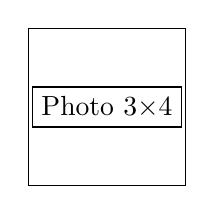
\begin{tikzpicture}
\begin{scope}[draw=black, yshift=2.5cm]
\draw (0,0) rectangle node[draw] {Photo 3$\times$4} ++(2,2); 
\end{scope}
\end{tikzpicture}
} \\
Alamat (Rumah asal)		& : & \@alamat & \\
Tempat/tanggal lahir	& : & \@tmplahir, \@tgllahir & \\			
Agama					& : & \@agama & \\
Telpon					& : & 1. Rumah : \@noRumah & \\
						&   & 2. Kantor : \@noKantor & \\
						&   & 3. HP : \@noHP & \\
E-mail					& : & \@email & \\
Status					& : & a. Belum Nikah b. Nikah & \\
No. Mahasiswa			& : & \@idnum & \\
Masuk S2				& : & \@mastermasuk & \\
						& : & Th. Akademik \@thakademikmasuk \space Semester ke-\@semestermasuk & \\
Lulus S2				& : & \@masterlulus & \\
						& : & Th. Akademik \@thakademiklulus \space Semester ke-\@semesterlulus & \\
Judul Tesis				& : & \multicolumn{2}{p{10cm}}{\@titleind} \\
						& : & \multicolumn{2}{p{10cm}}{\@titleeng} \\
TOEFL					& : & \@nilaiTestEnglish \space pada tahun \@tahunTest & \\
Pekerjaan				& : & \@job & \\
Instansi				& : & \@instansi & \\
Alamat Instansi			& : & \@instansialamat & \\
Telp.					& : & \@instansitelp & \\
\end{tabular}
\end{center}
\renewcommand{\arraystretch}{1}

\vspace{1cm}
\noindent
\begin{tabular}{p{9.5cm}p{8cm}}
\multirow{6}{*}{
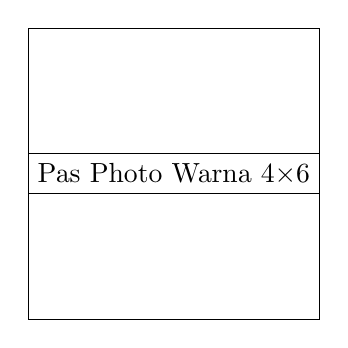
\begin{tikzpicture}
\begin{scope}[draw=black, yshift=2.5cm]
\draw (0,0) rectangle node[draw] (A) {Pas Photo Warna 4$\times$6} ++(3.7,3.7); 
\end{scope}
\end{tikzpicture}
}	& \@city,\space\today \\
	& Mahasiswa yang bersangkutan, \\ [2cm]
	& (\@fullname)
\end{tabular}

%%% permohonan yudisium
\newpage
\newgeometry{top=2cm,bottom=0.1cm}
\renewcommand{\arraystretch}{1.2}
\begin{tabular}{p{1.7cm}m{13cm}}
\multirow{3}{*}{
\includegraphics[width=1.6cm]{logougm}} 	
& \textbf{UNIVERSITAS GADJAH MADA} \\
& \textbf{FAKULTAS MATEMATIKA DAN ILMU PENGETAHUAN ALAM} \\
& \small \textbf{\textit{Kotak Pos BLS 21, Yogyakarta 55281 Telp. (0274) 513339, 902364}} 
\end{tabular}

\normalsize
\vspace{1cm}
\renewcommand{\arraystretch}{1}
\begin{tabular}{lp{.01cm}m{2.5cm}p{.01cm}m{6.1cm}}
Tanggal		& :	& \multicolumn{3}{l}{\today} \\
Lampiran	& : & \multicolumn{3}{l}{1 berkas} \\
Hal			& :	& \multicolumn{3}{l}{Permohonan Yudisium S2} \\ [.5cm]
Kepada Yth.	& :	& \multicolumn{3}{l}{Dekan} \\
			&	& \multicolumn{3}{l}{\@faculty} \\
			&	& \multicolumn{3}{l}{\@university} \\
			&	& \multicolumn{3}{l}{\@city} \\ [1cm]
			&	& \multicolumn{3}{l}{Dengan hormat,} \\ [.3cm]
			&	& \multicolumn{3}{l}{Yang bertanda tangan dibawah ini saya:} \\ [.2cm]
			&	& Nama			& :	& \@fullname \\ [.1cm]
			&	& NIM			& :	& \@idnum \\ [.1cm]
			&	& Jurusan		& :	& \@jurusan \\ [.1cm]
			&	& Program Studi	& :	& \@program \\ 
			&	&				&	& \\
			&	& \multicolumn{3}{l}{Mengajukan Permohonan untuk dinyatakan lulus S2 \@program.} \\ [.2cm]
			&	& \multicolumn{3}{l}{Atas perhatiannya, saya ucapkan terima kasih.}	
\end{tabular}

\vspace{1cm}
\begin{tabular}{p{10cm}p{10cm}}
Mengetahui,							&  \\
Ketua Program Studi Monodisiplin	& Pemohon, \\ 
\@program							& \\ [1.5cm]
\underline{\@headprogram}			& \@fullname \\
\@headprogramnip					& %NIM. \@idnum
\end{tabular}

%%%rekaputulasi hasil studi
\newpage
\newgeometry{top=2cm,bottom=0.1cm}
\renewcommand{\arraystretch}{1.2}
\begin{tabular}{p{1.7cm}m{13cm}}
\multirow{3}{*}{
\includegraphics[width=1.6cm]{logougm}} 	
& \textbf{UNIVERSITAS GADJAH MADA} \\
& \textbf{FAKULTAS MATEMATIKA DAN ILMU PENGETAHUAN ALAM} \\
& \small \textbf{\textit{Kotak Pos BLS 21, Yogyakarta 55281 Telp. (0274) 513339, 902364}} 
\end{tabular}

\vspace{1cm}
\begin{center}
{\normalfont\large\bfseries\expandafter{REKAPITULASI HASIL STUDI UNTUK YUDISIUM S2}}
\par\nobreak
\end{center}

\normalsize
\vspace{1cm}
\renewcommand{\arraystretch}{1.2}
\begin{tabular}{lp{0.01cm}m{5cm}}
Nama Mahasiswa				& :	& \@fullname \\
Nomor Mahasiswa				& :	& \@idnum \\
Angkatan					& :	& 2015 / 2016, Semester 5 \\
Program Studi				& :	& \@program \\
							&	& \\
Jml. sks sebelum pembatalan	& :	& \@sksbatalsebelum \\
Jumlah sks dibatalkan		& :	& \@sksbatal \\
Jml sks sesudah pembatalan	& :	& \@sksbatalsesudah \\
Jumlah sks dengan nilai D	& :	& \@sksD \\
							&	& \\
IPK sebelum Pembatalan		& :	& ....... \\
IPK sesudah Pembatalan		& :	& .......  			
\end{tabular}

\vspace{1cm}
\renewcommand{\arraystretch}{1}
\begin{tabular}{p{4cm}p{5cm}p{6cm}}
&							& Yogyakarta, \today \\
&							& \\
&							& Ketua Program Studi Monodisiplin \\
Mhs Ybs,		& Dicek Petugas Prodi S2,	& \@program \\
				&							& \\ [1.5cm]
\@fullname 		& \@adminS2ILKOM			& \underline{\@headprogram} \\
				&							& \@headprogramnip
\end{tabular}
\restoregeometry


%%% naskah publikasi
\newpage
\begin{singlespace}
\begin{center}
\large{NASKAH PUBLIKASI} \\

\vspace{5cm}
Untuk Berkala Penelitian Pascasarjana ini \\
Telah Disetujui oleh Pembimbing \\
\end{center}

\vspace{8cm}
\noindent
\textbf{Pembimbing} \\

\vspace{1.5cm}
\noindent
\textbf{\underline{\@firstsupervisor}} \hfill Tanggal, \today  \\
\textbf{\@firstsupervisornip}
\end{singlespace}

%%% Lembar persetujuan
\newpage
\begin{singlespace}
\begin{center}
\large{LEMBAR PERSETUJUAN} \\

\vspace{2.5cm}
\normalfont\@titleind \par\nobreak

\vspace{5cm}
\underline{\@fullname} \\
\@idnum \\
\end{center}

\vspace{4cm}
\noindent
\textbf{Disetujui oleh} \\
\textbf{Pembimbing} \\

\vspace{1.5cm}
\noindent
\textbf{\underline{\@firstsupervisor}} \hfill Tanggal, \today \\
\textbf{\@firstsupervisornip}
\end{singlespace}

%%% Lembar persetujuan inggris
\newpage
\begin{singlespace}
\begin{center}
\large{APPROVAL OF THE ADVISOR} \\

\vspace{2.5cm}
\normalfont\@titleeng \par\nobreak

\vspace{5cm}
\underline{\@fullname} \\
\@idnum \\
\end{center}

\vspace{4cm}
\noindent
\textbf{Approved by} \\
\textbf{Supervisor} \\

\vspace{1.5cm}
\noindent
\textbf{\underline{\@firstsupervisor}} \hfill Date: \@dateapprove  \\
\textbf{\@firstsupervisornip}
\end{singlespace}

%%% Surat pernyataan penyantuman nama pembimbing
\newpage
\onehalfspacing
\newgeometry{left=4cm,right=4cm}
\begin{center}
{\normalfont\large\bfseries\expandafter{PERNYATAAN}}
\par\nobreak
\end{center}

\vspace{1.0cm}
\noindent
Dengan ini kami selaku pembimbing tesis mahasiswa Program Pascasarjana: \\

\renewcommand{\arraystretch}{1.2}
\noindent
\begin{tabular}{p{2.5cm}p{0.01cm}p{5cm}}
Nama 			& : &\@fullname \\
NIM				& : &\@idnum \\
Program Studi	& : &\@program 
\end{tabular}

\vspace{0.3cm}
\noindent
\onehalfspacing
Setuju/tidak setuju *) naskah ringkasan penelitian (calon naskah berkala penelitian Program Pascasarjana yang disusun oleh yang bersangkutan dipublikasikan dengan/ tanpa *) mencantumkan  nama tim pembimbing sebagai \textit{co-author}.

\vspace{.3cm}
\noindent
Kemudian harap maklum.

\vspace{.5cm}
\singlespacing
\renewcommand{\arraystretch}{1.3}
\noindent
\begin{tabular}{p{2.5cm}p{.3cm}cp{.3cm}p{3cm}}
\multicolumn{5}{r}{Yogyakarta, \today} \\
\multicolumn{1}{l}{Nama} & & Status Pembimbing & &\multicolumn{1}{c}{Tanda Tangan} \\ [1.5cm]
\multicolumn{1}{l}{\textbf{\@firstsupervisor}} & & \textbf{Pembimbing Utama} & & \\ \cline{1-1} \cline{5-5}
\multicolumn{1}{l}{\textbf{\@firstsupervisornip}} & & \\
\end{tabular}

\vfill

\begin{footnotesize}
\begin{tabbing}
Ketera\=ngan:  \\
*) 	\> Coret yang tidak perlu
\end{tabbing}
\end{footnotesize}
\restoregeometry
%%%%%%%%%%%%%%%%%%%%%%%

%%%%%%%%%%%%%%%%%%%%%%% PERNYATAAN BEBAS PERPUS
\newpage
\onehalfspacing
\begin{center}
{\normalfont\large\bfseries\expandafter{\underline{SURAT PERNYATAAN}}}
\par\nobreak
\end{center}

\vspace{1.0cm}
\noindent
Saya yang bertandatangan dibawah ini: \\

\renewcommand{\arraystretch}{1.2}
\begin{tabular}{p{2.5cm}p{0.01cm}p{9cm}}
Nama 			& : &\@fullname \\
NIM				& : &\@idnum \\
Program Studi	& : &\@program \\	
No. HP			& : & \@noHP \\%0853 2948 3423 \\	
\end{tabular}

\vspace{0.3cm}
\noindent
Menyatakan dengan sesungguhnya bahwa saya tidak mempunyai tanggungan pinjaman berupa:

\vspace{0.2cm}
\begin{enumerate}
\item Buku Perpustakaan Pusat UGM
\item Buku Perpustakaan Fakultas/Program Studi
\item Alat Laboratorium (LPPT dan Program Studi)
\end{enumerate}

\vspace{0.2cm}
\noindent
Surat pernyataan ini dibuat untuk persyaratan wisuda program Pascasarjana Universitas Gadjah Mada, dan apabila tidak benar, maka saya bersedia menerima sanksi.

\vspace{1cm}
\singlespacing
\noindent
\begin{tabular}{p{9.5cm}p{5cm}}
	& \@city,\space\today \\
	& Yang menyatakan, \\
	& \multicolumn{1}{l}{
	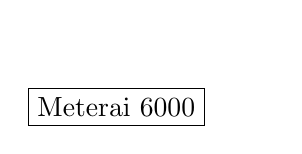
\begin{tikzpicture}
	\draw (0,0) node[draw] {Meterai 6000} ++(2,1); 
	\end{tikzpicture}
	} \\ [1cm]
	& \@fullname
\end{tabular}
%%%%%%%%%%%%%%%%%%%%%%%

%%%%%%%%%%%%%%%%%%%%%%% Surat penghapusan mata kuliah
\newpage
\onehalfspacing
\begin{center}
{\normalfont\large\bfseries\expandafter{SURAT PERMOHONAN PENGHAPUSAN MATA KULIAH}}
\par\nobreak
\end{center}

\vspace{1.0cm}
\noindent
Kepada Yth. \\
Ketua Program Studi \@program \\ \@headprogram \\ Di Yogyakarta

\vspace{0.5cm}
\noindent
Dengan hormat,\\
Saya yang bertanda tangan di bawah ini:

\singlespacing
\begin{tabular}{p{3.5cm}p{0.01cm}p{9cm}}
Nama 			& : & \@fullname \\
Nomor Mahasiswa	& : & \@idnum \\
Program Studi	& : & \@program \\				
Angkatan		& : & \@angkatan
\end{tabular}

\onehalfspacing
\vspace{0.3cm}
\noindent
Mengajukan permohonan penghapusan mata kuliah pada semester genap tahun akademik 2016/2017 dengan rincian dibawah ini:

\vspace{0.2cm}
\begin{center}
\begin{tabular}{|p{0.3cm}|p{5cm}|p{3cm}|p{4cm}|}
\hline
\multicolumn{1}{|c|}{No} & \multicolumn{1}{c|}{Mata Kuliah} & \multicolumn{1}{c|}{Kode MK} & \multicolumn{1}{c|}{Nilai} \\ \hline
\multicolumn{1}{|c|}{1}  & PENGENALAN POLA & \multicolumn{1}{c|}{CS6834} & \multicolumn{1}{c|}{B/C} \\ \hline
\end{tabular}
\end{center}

\vspace{0.2cm}
\noindent
Dengan alasan jumlah total SKS yang telah saya tempuh melebihi yang disyaratkan, sehingga dengan adanya pembatalan matakuliah pilihan tersebut diatas dapat meningkatkan nilai indeks prestasi kumulatif (IPK).

\vspace{.2cm}
\noindent
Demikian surat permohonan ini saya buat dengan sebenarnya, atas perhatian dan kesediaannya, saya ucapkan terima kasih.

\vspace{0.5cm}
\singlespacing
\noindent
\begin{tabular}{p{10cm}p{10cm}}
Mengetahui,							& \@city,\space\today \\
Ketua Program Studi \@program		& Pemohon, \\ [1.5cm]
\underline{\@headprogram}			& \@fullname \\
\@headprogramnip					& %NIM. \@idnum
\end{tabular}
%%%%%%%%%%%%%%%%%%%%%%%

%%% permohonan refund
\newpage
\renewcommand{\arraystretch}{1}
\begin{tabular}{lp{.01cm}m{2.5cm}p{.01cm}p{7cm}}
Hal			& :	& \multicolumn{3}{l}{\textbf{\textit{Permohonan Refund SPP}}} \\ [.5cm]
Kepada Yth.	& :	& \multicolumn{3}{l}{Yth. Dekan} \\
			&	& \multicolumn{3}{l}{\textit{u.b} Wakil Dekan Bidang Akademik dan Kemahasiswaan} \\
			&	& \multicolumn{3}{l}{\@faculty} \\
			&	& \multicolumn{3}{l}{\@university} \\ [1cm]
			&	& \multicolumn{3}{l}{Dengan hormat,} \\ [.3cm]
			&	& \multicolumn{3}{l}{Yang bertanda tangan dibawah ini saya:} \\ [.2cm]
			&	& Nama			& :	& \@fullname \\ [.1cm]
			&	& NIM			& :	& \@idnum \\ [.1cm]
			&	& Departemen	& :	& \@dept \\ [.1cm]
			&	& Program Studi	& :	& \@program \\ [.1cm]
			&	& Alamat		& :	& \@alamat \\ [.1cm]					&	& No. HP		& :	& \@noHP \\ 
			&	&				&	& \\
			&	& \multicolumn{3}{p{12cm}}{Dengan ini saya mengajukan permohonan refund SPP karena telah berakhirnya masa studi saya.} \\ [.2cm]
			&	& \multicolumn{3}{p{12cm}}{Demikian surat permohonan ini saya buat, atas  terkabulnya  permohonan   ini saya ucapkan terima kasih.}	
\end{tabular}

\vspace{1cm}
\begin{center}
\begin{tabular}{p{11cm}p{4cm}}
							& \@city, \today \\
Dosen Pembimbing,			& Pemohon, \\ [1.5cm]
\underline{\@firstsupervisor}			& \@fullname \\
\@firstsupervisornip					& \\ [.5cm] 
\multicolumn{2}{c}{Megetahui,} \\
\multicolumn{2}{c}{Pengelola Program Studi \@program} \\ [1.5cm]
\multicolumn{2}{c}{\underline{\@headprogram}} \\
\multicolumn{2}{c}{\@headprogramnip} 
\end{tabular}
\end{center}
